\documentclass[11pt,]{article}
\usepackage[]{mathpazo}
\usepackage{amssymb,amsmath}
\usepackage{ifxetex,ifluatex}
\usepackage{fixltx2e} % provides \textsubscript
\ifnum 0\ifxetex 1\fi\ifluatex 1\fi=0 % if pdftex
  \usepackage[T1]{fontenc}
  \usepackage[utf8]{inputenc}
\else % if luatex or xelatex
  \ifxetex
    \usepackage{mathspec}
  \else
    \usepackage{fontspec}
  \fi
  \defaultfontfeatures{Ligatures=TeX,Scale=MatchLowercase}
\fi
% use upquote if available, for straight quotes in verbatim environments
\IfFileExists{upquote.sty}{\usepackage{upquote}}{}
% use microtype if available
\IfFileExists{microtype.sty}{%
\usepackage{microtype}
\UseMicrotypeSet[protrusion]{basicmath} % disable protrusion for tt fonts
}{}
\usepackage[margin=1in]{geometry}
\usepackage{hyperref}
\hypersetup{unicode=true,
            pdftitle={Understanding Data and its Environment: Report assessment},
            pdfauthor={Eugeni Vidal},
            pdfborder={0 0 0},
            breaklinks=true}
\urlstyle{same}  % don't use monospace font for urls
\usepackage{color}
\usepackage{fancyvrb}
\newcommand{\VerbBar}{|}
\newcommand{\VERB}{\Verb[commandchars=\\\{\}]}
\DefineVerbatimEnvironment{Highlighting}{Verbatim}{commandchars=\\\{\}}
% Add ',fontsize=\small' for more characters per line
\usepackage{framed}
\definecolor{shadecolor}{RGB}{248,248,248}
\newenvironment{Shaded}{\begin{snugshade}}{\end{snugshade}}
\newcommand{\KeywordTok}[1]{\textcolor[rgb]{0.13,0.29,0.53}{\textbf{{#1}}}}
\newcommand{\DataTypeTok}[1]{\textcolor[rgb]{0.13,0.29,0.53}{{#1}}}
\newcommand{\DecValTok}[1]{\textcolor[rgb]{0.00,0.00,0.81}{{#1}}}
\newcommand{\BaseNTok}[1]{\textcolor[rgb]{0.00,0.00,0.81}{{#1}}}
\newcommand{\FloatTok}[1]{\textcolor[rgb]{0.00,0.00,0.81}{{#1}}}
\newcommand{\ConstantTok}[1]{\textcolor[rgb]{0.00,0.00,0.00}{{#1}}}
\newcommand{\CharTok}[1]{\textcolor[rgb]{0.31,0.60,0.02}{{#1}}}
\newcommand{\SpecialCharTok}[1]{\textcolor[rgb]{0.00,0.00,0.00}{{#1}}}
\newcommand{\StringTok}[1]{\textcolor[rgb]{0.31,0.60,0.02}{{#1}}}
\newcommand{\VerbatimStringTok}[1]{\textcolor[rgb]{0.31,0.60,0.02}{{#1}}}
\newcommand{\SpecialStringTok}[1]{\textcolor[rgb]{0.31,0.60,0.02}{{#1}}}
\newcommand{\ImportTok}[1]{{#1}}
\newcommand{\CommentTok}[1]{\textcolor[rgb]{0.56,0.35,0.01}{\textit{{#1}}}}
\newcommand{\DocumentationTok}[1]{\textcolor[rgb]{0.56,0.35,0.01}{\textbf{\textit{{#1}}}}}
\newcommand{\AnnotationTok}[1]{\textcolor[rgb]{0.56,0.35,0.01}{\textbf{\textit{{#1}}}}}
\newcommand{\CommentVarTok}[1]{\textcolor[rgb]{0.56,0.35,0.01}{\textbf{\textit{{#1}}}}}
\newcommand{\OtherTok}[1]{\textcolor[rgb]{0.56,0.35,0.01}{{#1}}}
\newcommand{\FunctionTok}[1]{\textcolor[rgb]{0.00,0.00,0.00}{{#1}}}
\newcommand{\VariableTok}[1]{\textcolor[rgb]{0.00,0.00,0.00}{{#1}}}
\newcommand{\ControlFlowTok}[1]{\textcolor[rgb]{0.13,0.29,0.53}{\textbf{{#1}}}}
\newcommand{\OperatorTok}[1]{\textcolor[rgb]{0.81,0.36,0.00}{\textbf{{#1}}}}
\newcommand{\BuiltInTok}[1]{{#1}}
\newcommand{\ExtensionTok}[1]{{#1}}
\newcommand{\PreprocessorTok}[1]{\textcolor[rgb]{0.56,0.35,0.01}{\textit{{#1}}}}
\newcommand{\AttributeTok}[1]{\textcolor[rgb]{0.77,0.63,0.00}{{#1}}}
\newcommand{\RegionMarkerTok}[1]{{#1}}
\newcommand{\InformationTok}[1]{\textcolor[rgb]{0.56,0.35,0.01}{\textbf{\textit{{#1}}}}}
\newcommand{\WarningTok}[1]{\textcolor[rgb]{0.56,0.35,0.01}{\textbf{\textit{{#1}}}}}
\newcommand{\AlertTok}[1]{\textcolor[rgb]{0.94,0.16,0.16}{{#1}}}
\newcommand{\ErrorTok}[1]{\textcolor[rgb]{0.64,0.00,0.00}{\textbf{{#1}}}}
\newcommand{\NormalTok}[1]{{#1}}
\usepackage{graphicx,grffile}
\makeatletter
\def\maxwidth{\ifdim\Gin@nat@width>\linewidth\linewidth\else\Gin@nat@width\fi}
\def\maxheight{\ifdim\Gin@nat@height>\textheight\textheight\else\Gin@nat@height\fi}
\makeatother
% Scale images if necessary, so that they will not overflow the page
% margins by default, and it is still possible to overwrite the defaults
% using explicit options in \includegraphics[width, height, ...]{}
\setkeys{Gin}{width=\maxwidth,height=\maxheight,keepaspectratio}
\IfFileExists{parskip.sty}{%
\usepackage{parskip}
}{% else
\setlength{\parindent}{0pt}
\setlength{\parskip}{6pt plus 2pt minus 1pt}
}
\setlength{\emergencystretch}{3em}  % prevent overfull lines
\providecommand{\tightlist}{%
  \setlength{\itemsep}{0pt}\setlength{\parskip}{0pt}}
\setcounter{secnumdepth}{5}
% Redefines (sub)paragraphs to behave more like sections
\ifx\paragraph\undefined\else
\let\oldparagraph\paragraph
\renewcommand{\paragraph}[1]{\oldparagraph{#1}\mbox{}}
\fi
\ifx\subparagraph\undefined\else
\let\oldsubparagraph\subparagraph
\renewcommand{\subparagraph}[1]{\oldsubparagraph{#1}\mbox{}}
\fi

%%% Use protect on footnotes to avoid problems with footnotes in titles
\let\rmarkdownfootnote\footnote%
\def\footnote{\protect\rmarkdownfootnote}

%%% Change title format to be more compact
\usepackage{titling}

% Create subtitle command for use in maketitle
\newcommand{\subtitle}[1]{
  \posttitle{
    \begin{center}\large#1\end{center}
    }
}

\setlength{\droptitle}{-2em}
  \title{Understanding Data and its Environment: Report assessment}
  \pretitle{\vspace{\droptitle}\centering\huge}
  \posttitle{\par}
  \author{Eugeni Vidal}
  \preauthor{\centering\large\emph}
  \postauthor{\par}
  \predate{\centering\large\emph}
  \postdate{\par}
  \date{March 15, 2018}


\begin{document}
\maketitle

{
\setcounter{tocdepth}{2}
\tableofcontents
}
\pagebreak

\section{Introduction}\label{introduction}

The Cambridge English Dictionary (2018) describes sales forecasting as
``the statement of what the amount or value of a company's sales is
likely to be in the future, based on information available now about the
market, past sales, etc''.

The increase of competition, complexity in business tasks, and the fact
that nowadays circumstances, in general, tend to change more rapidly
makes increasingly important and necessary for companies the use of
forecasting technics for the prediction of their future prospects
(Lancaster and Lomas 1985, 1).

 This report aims to describe, pre-process and analyse a set of data
based on historical sales data collected from a nationwide retailer in
the U.S as well as on external factors, so as to lead to the development
of an accurate predictive model.

 The methodology followed is divided into 7 different steps, from
describing the data to building and assessing the model developed (see
figure 1). Notice that although each step is taken in order, the whole
process has to be understood as a set of nested loops rather than a
straight line.

\begin{figure}[htbp]
\centering
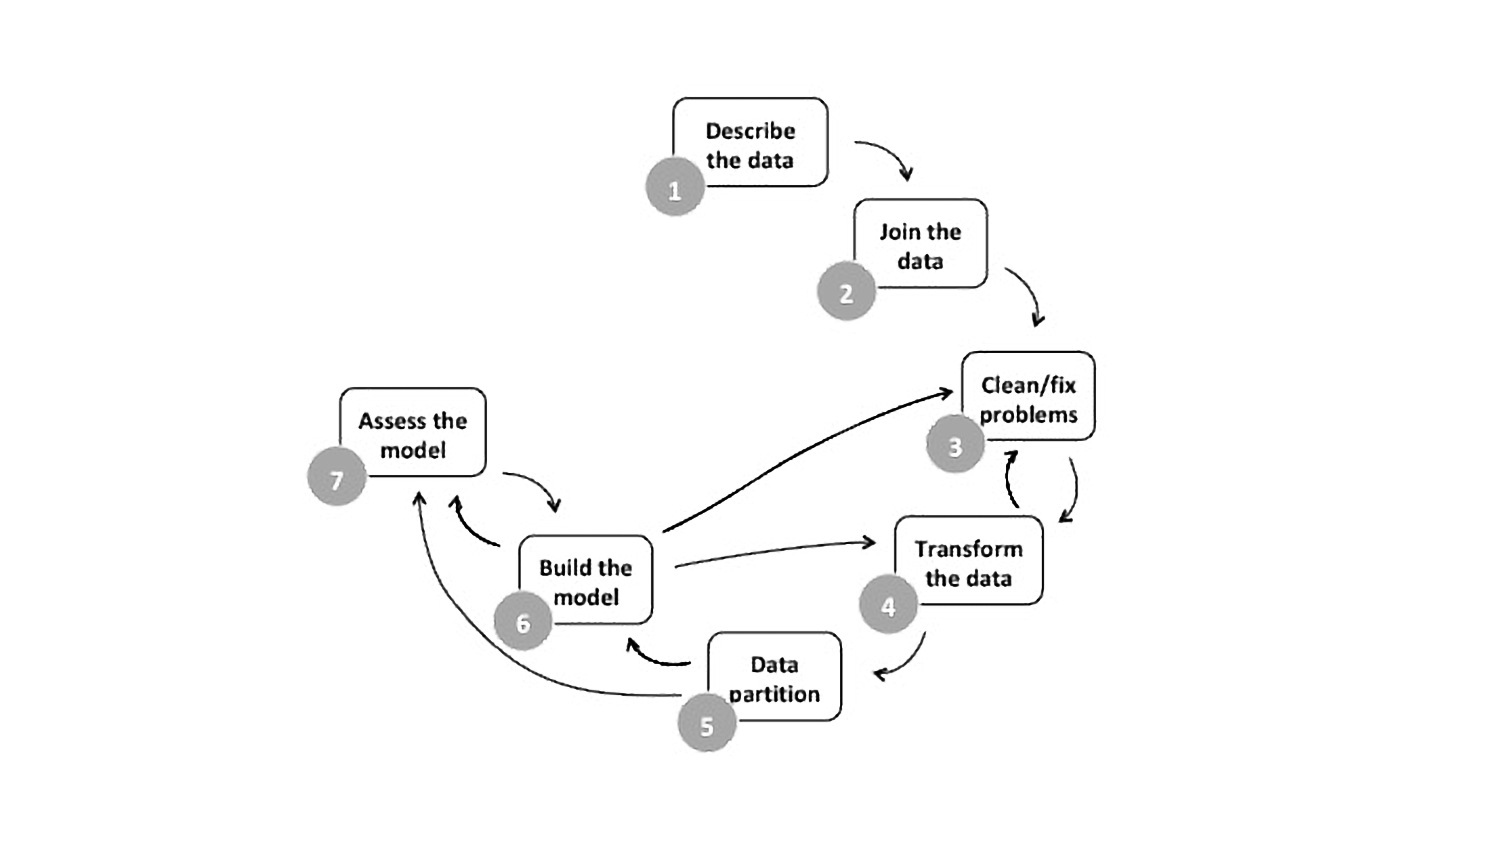
\includegraphics{images/Methodology diagram.v1.jpg}
\caption{Methodology diagram \label{}}
\end{figure}

The whole process has been done using the open software R and it is
reproducible based on code available at
\url{https://github.com/eugenividal/Understanding-data-report}.

This report is written as clearly and easily as possible, with the
pretense that any person, without much prior knowledge in forecasting or
in the R software, can understand it. For this purpose, the document
describes not only the statistical process followed, but also the code
used with the software R to carry it out.

\section{Data description}\label{data-description}

First of all, we will install the required packages and will activate
their libraries.

\begin{Shaded}
\begin{Highlighting}[]
\CommentTok{# Activate libraries}
\KeywordTok{library}\NormalTok{(tidyverse)}
\KeywordTok{library}\NormalTok{(VIM)}
\KeywordTok{library}\NormalTok{(ggplot2)}
\KeywordTok{library}\NormalTok{(dplyr)}
\KeywordTok{library}\NormalTok{(psych)}
\KeywordTok{library}\NormalTok{(lubridate)}
\KeywordTok{library}\NormalTok{(caret)}
\KeywordTok{library}\NormalTok{(car)}
\end{Highlighting}
\end{Shaded}

Secondly, we will load the data into the R environment.

\begin{Shaded}
\begin{Highlighting}[]
\CommentTok{# Load data}
\NormalTok{stores =}\StringTok{ }\KeywordTok{read_csv}\NormalTok{(}\StringTok{"data/stores.csv"}\NormalTok{)}
\NormalTok{features =}\StringTok{ }\KeywordTok{read_csv}\NormalTok{(}\StringTok{"data/features.csv"}\NormalTok{)}
\NormalTok{test =}\StringTok{ }\KeywordTok{read_csv}\NormalTok{(}\StringTok{"data/test.csv"}\NormalTok{)}
\NormalTok{train =}\StringTok{ }\KeywordTok{read_csv}\NormalTok{(}\StringTok{"data/train.csv"}\NormalTok{)}
\end{Highlighting}
\end{Shaded}

We are provided with 4 data sets (stores, features, train, and test).
All of them with the same format: comma-separated values (csv).

Here is a brief description of each of the datasets and their variables:

\textbf{stores.csv (45 obs. of 3 variables)}

\begin{itemize}
\tightlist
\item
  Store: the anonymised store number 
\item
  Type: tore type, A: supercentre, B: superstore, C: supermarket 
\item
  Size (sq ft): store size (in square feet) 
\end{itemize}

\textbf{features.csv (8,190 obs. of 12 variables)}

\begin{itemize}
\tightlist
\item
  Store: the anonymised store number 
\item
  Date: the week with the dated Friday 
\item
  Temperature: average temperature in the region 
\item
  Fuel\_Price: cost of fuel in the region 
\item
  Promotions: anonymised data related to promotions, mainly price
  reductions that the retailer is running 
\item
  CPI: the consumer price index 
\item
  Unemployment: the unemployment rate 
\item
  IsHoliday: whether the week is a special holiday week 
\end{itemize}

\textbf{train.csv (421,570 obs. of 5 variables)}

\begin{itemize}
\tightlist
\item
  Store: the anonymised store number 
\item
  Department: the anonymised department number 
\item
  Date: the week with the dated Friday 
\item
  Weekly\_Sales: sales for the given department in the given store 
\item
  IsHoliday: whether the week is a special holiday week 
\end{itemize}

\textbf{test.csv (115,069 obs. of 5 variables)}

The validation dataset has the same fields as the train.csv, except we
need to predict the weekly sales for each triplet of store, department,
and date from 02/11/2012 to 26/07/2013.

Variables of each dataset have been explored through counts, summary
statistics, crosstabulation and visualisations in order to identify
potential inconsistences or problems.

The main issues detected are briefly described below.

\textbf{1. Inconsistent data encoding}. In the stores dataset, some
stores might be wrongly classified. Two stores under 50,000 sq ft are
coded as type B and other two as type A, when presumably small size
stores (\textless{}50000 sq ft) should be type C.

\textbf{2. Missing values}. In the features dataset, 24,040 values are
missing, almost 50\% in the promotion variables and 7\% in the
\texttt{CPI} and \texttt{Unemployment} ones. With the function of the
VIM package \texttt{aggr()} we can visualise them for each variable
alone and for each combination of variables. There are no missing values
in the rest of datasets.

\begin{Shaded}
\begin{Highlighting}[]
\CommentTok{# Plot missing values}
\KeywordTok{aggr}\NormalTok{(features, }\DataTypeTok{prop =} \OtherTok{FALSE}\NormalTok{, }\DataTypeTok{col =} \StringTok{"grey"}\NormalTok{, }\DataTypeTok{cex.lab =} \FloatTok{0.85}\NormalTok{, }\DataTypeTok{cex.axis =} \FloatTok{0.65}\NormalTok{, }
    \DataTypeTok{cex.main =} \FloatTok{0.85}\NormalTok{)}
\end{Highlighting}
\end{Shaded}

\begin{figure}[htbp]
\centering
\includegraphics{REPORTv12_files/figure-latex/unnamed-chunk-6-1.pdf}
\caption{Missing values}
\end{figure}

\textbf{3. Negative values}. Some of the values in the promotions
variables are negative: 4 in \texttt{Promotion1}, 25 in
\texttt{Promotion2}, 13 in \texttt{Promotion3}, and 2 in
\texttt{Promotion5}. Also \texttt{Weekly\ Sales} in the train dataset
has some negative values (1286 out of 421571 (0.3\%)).

\textbf{4. Class type errors}. The class of the \texttt{Date} variable
within the train, features and test datasets is character instead of
date. This doesn't allow to sort the data properly. Also in terms of
class, it would be useful to have the variable IsHoliday in numeric type
(1 or 0) instead of boolean (true or false).

\textbf{5. Data not normally distributed}. The data in some variables is
not normally distributed. \texttt{Weekly\_Sales} data is clearly
left-skewed (see histogram below), \texttt{Size\_(sq\ ft)} rather comb,
and \texttt{Fuel\_Price} and \texttt{CPI} bimodal.

\begin{Shaded}
\begin{Highlighting}[]
\CommentTok{# Plot a histogram}
\KeywordTok{ggplot}\NormalTok{(}\DataTypeTok{data =} \NormalTok{train, }\KeywordTok{aes}\NormalTok{(train$Weekly_Sales)) +}\StringTok{ }\KeywordTok{geom_histogram}\NormalTok{(}\KeywordTok{aes}\NormalTok{(), }
    \DataTypeTok{alpha =} \FloatTok{0.5}\NormalTok{) +}\StringTok{ }\KeywordTok{labs}\NormalTok{(}\DataTypeTok{x =} \StringTok{"Weekly Sales"}\NormalTok{, }\DataTypeTok{y =} \StringTok{"Frequency"}\NormalTok{) +}\StringTok{ }
\StringTok{    }\KeywordTok{theme_classic}\NormalTok{()}
\end{Highlighting}
\end{Shaded}

\begin{verbatim}
## `stat_bin()` using `bins = 30`. Pick better value with `binwidth`.
\end{verbatim}

\begin{figure}[htbp]
\centering
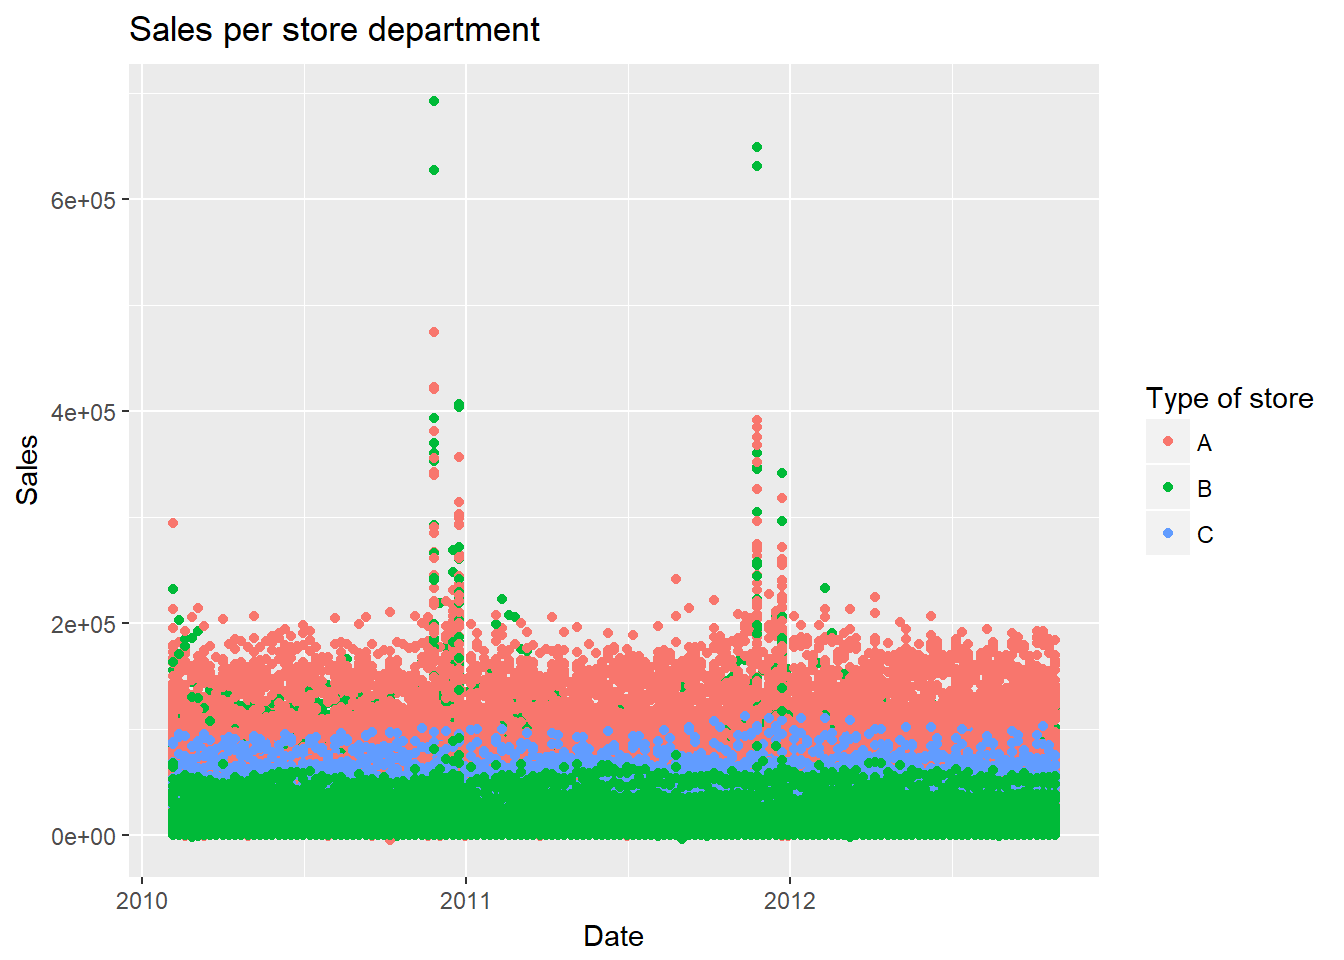
\includegraphics{REPORTv12_files/figure-latex/unnamed-chunk-8-1.pdf}
\caption{Weekly Sales histogram}
\end{figure}

\textbf{6. Extreme values}. Finally, to mention that some variables
present observations that could be considered as outliers or extreme. An
example are the stand out points shown below in the plot of weekly Sales
by date. We analise this later when building the model

\section{Data joining}\label{data-joining}

The next step is to join the stores, train and features datasets in a
single one. This will allow us to make the analysis simpler and more
straightforward.

The test dataset will be left aside to gauge the effectiveness of the
models once build.

To performance the join, we apply a left join. We chose this type of
join because we want to end up having the same number of rows as the
train dataset which contains the variable to predict
\texttt{Weekly\_Sales}.

First, we link the stores dataset with the train one, using the common
attribute \texttt{Store}; then the resultant dataset with the features
dataset, using the common attributes \texttt{Store}, \texttt{Date} and
\texttt{IsHoliday}.

\begin{Shaded}
\begin{Highlighting}[]
\CommentTok{# Join store-level data onto training dataset (so we know}
\CommentTok{# size and type)}
\NormalTok{data_joined =}\StringTok{ }\KeywordTok{left_join}\NormalTok{(train, }\DataTypeTok{y =} \NormalTok{stores)}
\end{Highlighting}
\end{Shaded}

\begin{verbatim}
## Joining, by = "Store"
\end{verbatim}

\begin{Shaded}
\begin{Highlighting}[]
\CommentTok{# Join train_joined onto features dataset (so we know the}
\CommentTok{# rest of variables)}
\NormalTok{data_joined =}\StringTok{ }\KeywordTok{left_join}\NormalTok{(data_joined, }\DataTypeTok{y =} \NormalTok{features)}
\end{Highlighting}
\end{Shaded}

\begin{verbatim}
## Joining, by = c("Store", "Date", "IsHoliday")
\end{verbatim}

The result is a data frame with 421,570 observations of 16 variables.
Notice that 1,755 observations don't match between train and features.
This is because we did a left join and the features datasets collects
observations for a longer period than the train dataset.

\section{Cleaning and fixing problems with the
data}\label{cleaning-and-fixing-problems-with-the-data}

In this section, we will clean or fix the inconsistencies or potential
problems identified in the section data description.

\subsection{Resolving inconsistent data
encoding}\label{resolving-inconsistent-data-encoding}

It is assumed that the type of store is based on size and consequently,
all stores under 50000 sq ft are recoded as C type. This way the
potential inconsistency of 4 stores under 5000 sq ft coded as type A and
B are solved.

\begin{Shaded}
\begin{Highlighting}[]
\CommentTok{# Recode `stores$Type` based on `stores$Size (sq ft)`}
\NormalTok{data_joined$Type[(data_joined$}\StringTok{`}\DataTypeTok{Size (sq ft)}\StringTok{`} \NormalTok{<}\StringTok{ }\DecValTok{50000}\NormalTok{)] <-}\StringTok{ "C"}
\NormalTok{data_joined$Type[(data_joined$}\StringTok{`}\DataTypeTok{Size (sq ft)}\StringTok{`} \NormalTok{>=}\StringTok{ }\DecValTok{50000}\NormalTok{) &}\StringTok{ }\NormalTok{(data_joined$}\StringTok{`}\DataTypeTok{Size (sq ft)}\StringTok{`} \NormalTok{<}\StringTok{ }
\StringTok{    }\DecValTok{150000}\NormalTok{)] <-}\StringTok{ "B"}
\NormalTok{data_joined$Type[(data_joined$}\StringTok{`}\DataTypeTok{Size (sq ft)}\StringTok{`} \NormalTok{>=}\StringTok{ }\DecValTok{150000}\NormalTok{)] <-}\StringTok{ "A"}
\end{Highlighting}
\end{Shaded}

\subsection{Dealing with missing
values}\label{dealing-with-missing-values}

There are several approaches to deal with this problem:

\begin{itemize}
\item
  delete the cases containing missing data (listwise deletion), or
\item
  replace (impute) the missing values with reasonable alternative data
  values (Kabacoff 2011, 353).
\end{itemize}

Deciding how to treat them will depend on the estimation of which
approach will produce the most reliable and accurate results (Kabacoff
2011, 354).

The amount of missing data is an important factor in this sense. There
is no established cutoff from the literature regarding an acceptable
percentage of missing data in a dataset for valid statistical inferences
(Dong and Peng 2013). Schafer (1999) argues that a missing rate of 5\%
or less is inconsequential, while Bennett (2001) considers that more
than 10\% is likely to biased the statistical analysis.

Given the high percentage of missing values in the promotion variables
(around 50\%), we will delete them and will not consider in the
statistical analysis.

\begin{Shaded}
\begin{Highlighting}[]
\CommentTok{# Delete promotions}
\NormalTok{data_joined$Promotion1 <-}\StringTok{ }\OtherTok{NULL}
\NormalTok{data_joined$Promotion2 <-}\StringTok{ }\OtherTok{NULL}
\NormalTok{data_joined$Promotion3 <-}\StringTok{ }\OtherTok{NULL}
\NormalTok{data_joined$Promotion4 <-}\StringTok{ }\OtherTok{NULL}
\NormalTok{data_joined$Promotion5 <-}\StringTok{ }\OtherTok{NULL}
\end{Highlighting}
\end{Shaded}

The missing data previously detected in the \texttt{CPI} and
\texttt{Unemployment} variables disappeared when the datasets were
joined With the left\_join.

\subsection{Negative values
interpretation}\label{negative-values-interpretation}

After analyzing the negative values of the \texttt{Weekly\_Sales}
variable, we have concluded that they are returned products from
previous weeks. So, no changes will be done in this sense.

The rest of the negative values were detected in the promotions
variables that we just deleted, so they are no longer a problem.

\subsection{Data type conversion}\label{data-type-conversion}

In order to make the variable \texttt{IsHoliday} more manageable, we
will convert the data type into numeric using the basic function
\texttt{as.numeric()}.

\begin{Shaded}
\begin{Highlighting}[]
\CommentTok{# Convert IsHoliday to numeric}
\NormalTok{data_joined$IsHoliday <-}\StringTok{ }\KeywordTok{as.numeric}\NormalTok{(data_joined$IsHoliday)}
\end{Highlighting}
\end{Shaded}

We will also convert the \texttt{Date} class from character into date
with the \texttt{mdy\ ()} function of the lubridate package.

\begin{Shaded}
\begin{Highlighting}[]
\CommentTok{# Convert date info to date format 'dmy'}
\NormalTok{data_joined$Date <-}\StringTok{ }\KeywordTok{dmy}\NormalTok{(data_joined$Date)}
\end{Highlighting}
\end{Shaded}

\subsection[Consideration of data
normalisation]{\texorpdfstring{Consideration of data
normalisation\footnote{The variables were normalised using log 10 during
  the process of building the model, but the results of the assesssment
  didn't imporve the model. This step is not explained in detail due to
  the limitation of words in the report}}{Consideration of data normalisation}}\label{consideration-of-data-normalisation}

It might be useful to have the errors normally distributed with constant
variance in order to produce prediction intervals, although it is not
considered necessary for forecasting (Hyndman and Athana­sopou­los
2017).

So, at this stage at least, all the variables will remain with their
original distribution. It could be preferable since the model would be
more understandable and interpretable1.

\subsection[Extreme values examination]{\texorpdfstring{Extreme values
examination\footnote{The extremes values were checked using a
  multivariate model apporach during the process of building the model,
  but their cleaning didn't influence on the regression model. So, we
  opt for keeping them. This step is not explained in detail due to the
  limitation of words in the report}}{Extreme values examination}}\label{extreme-values-examination}

No changes have been done in terms of extreme values at this stage. This
is cheked during the process of building the model using a multivariate
approach.

\section{Data transformation}\label{data-transformation}

Once the inconsistencies or potential problems are fixed, some
transformations are carried out in order to prepare the dataset for
building the model.

First, we will create a week number of year column in order to compare
them.

\begin{Shaded}
\begin{Highlighting}[]
\CommentTok{# Create a week number of the year variable}
\NormalTok{data_joined$WeekNum <-}\StringTok{ }\KeywordTok{as.numeric}\NormalTok{(}\KeywordTok{format}\NormalTok{(data_joined$Date +}\StringTok{ }\DecValTok{3}\NormalTok{, }\StringTok{"%U"}\NormalTok{))}
\end{Highlighting}
\end{Shaded}

Secondly, we will extract a year column from the date variable.

\begin{Shaded}
\begin{Highlighting}[]
\CommentTok{# Create a year variable}
\NormalTok{data_joined$year =}\StringTok{ }\NormalTok{lubridate::}\KeywordTok{year}\NormalTok{(data_joined$Date)}
\end{Highlighting}
\end{Shaded}

Finally, we will generate a variable of the previous year Weekly Sales.
As Zoltners et al argues (2001, 342) the current year sales can be a
very powerful predictor of the next year's sales.

\begin{Shaded}
\begin{Highlighting}[]
\CommentTok{# Create a previous year sales variable}
\NormalTok{prevyear =}\StringTok{ }\KeywordTok{select}\NormalTok{(data_joined, year, WeekNum, Dept, Store, }\DataTypeTok{prev_Weekly_Sales =} \NormalTok{Weekly_Sales)}
\NormalTok{prevyear$year =}\StringTok{ }\NormalTok{prevyear$year +}\StringTok{ }\DecValTok{1}
\CommentTok{# Create variable Sales previous year}
\NormalTok{data_joined =}\StringTok{ }\KeywordTok{left_join}\NormalTok{(data_joined, prevyear)}
\end{Highlighting}
\end{Shaded}

\begin{verbatim}
## Joining, by = c("Store", "Dept", "WeekNum", "year")
\end{verbatim}

The following figure shows how highly correlated are the weekly sales
variable of the previous year that we just created and the weekly sales
variable that we already had.

\begin{Shaded}
\begin{Highlighting}[]
\CommentTok{# Scatter plot Weekely Sales ~ Previous Year Weekly Sales}
\KeywordTok{ggplot}\NormalTok{(data_joined, }\KeywordTok{aes}\NormalTok{(}\DataTypeTok{x =} \NormalTok{Weekly_Sales, }\DataTypeTok{y =} \NormalTok{prev_Weekly_Sales)) +}\StringTok{ }
\StringTok{    }\KeywordTok{geom_point}\NormalTok{() +}\StringTok{ }\KeywordTok{labs}\NormalTok{(}\DataTypeTok{title =} \OtherTok{NULL}\NormalTok{, }\DataTypeTok{x =} \StringTok{"Weekly Sales"}\NormalTok{, }\DataTypeTok{y =} \StringTok{"Previous year Weekly Sales"}\NormalTok{) +}\StringTok{ }
\StringTok{    }\KeywordTok{theme_classic}\NormalTok{()}
\end{Highlighting}
\end{Shaded}

\begin{verbatim}
## Warning: Removed 160029 rows containing missing values (geom_point).
\end{verbatim}

\includegraphics{REPORTv12_files/figure-latex/unnamed-chunk-18-1.pdf}

Due to the fact that the new variable is based on sales of a previous
year, there will have a year of missing values.

We will handle with this applying again listwise deletion. This will
reduce the sample size by 38\% (from 421,570 to 261,541) which could
reduce statistical power of our model dataset. However, an approach with
the entire dataset could bias the results of the subsequent analysis
(Bennett 2001, 464).

\begin{Shaded}
\begin{Highlighting}[]
\CommentTok{# Delete rowns with NA's}
\NormalTok{data_joined =}\StringTok{ }\KeywordTok{na.omit}\NormalTok{(data_joined)}
\end{Highlighting}
\end{Shaded}

\section{Data partition}\label{data-partition}

In this section, the model dataset data\_joined is divided into two
parts. The first one, the training set (data\_joinedT), will be used to
build the model; the second one, the validation set (data\_joinedV), to
adjust it.

For the partition, we will use the \texttt{caret} package.

\begin{Shaded}
\begin{Highlighting}[]
\CommentTok{# subset the data into train and test}
\NormalTok{n =}\StringTok{ }\KeywordTok{nrow}\NormalTok{(data_joined)}
\NormalTok{trainIndex =}\StringTok{ }\KeywordTok{sample}\NormalTok{(}\DecValTok{1}\NormalTok{:n, }\DataTypeTok{size =} \KeywordTok{round}\NormalTok{(}\FloatTok{0.8} \NormalTok{*}\StringTok{ }\NormalTok{n), }\DataTypeTok{replace =} \OtherTok{FALSE}\NormalTok{)}
\NormalTok{data_joinedT =}\StringTok{ }\NormalTok{data_joined[trainIndex, ]}
\NormalTok{data_joinedV =}\StringTok{ }\NormalTok{data_joined[-trainIndex, ]}
\end{Highlighting}
\end{Shaded}

\section{Building the model}\label{building-the-model}

To build the model, we first choose the forecasting technique, then
analyse which predictors are more influencal for the prediction, and
finallly obtain a specific model, which best explain how sales will be
in the future.

\subsection{The choice of the
technique}\label{the-choice-of-the-technique}

The choice of forecasting technique is a major consideration. There are
many different methods to apply, from pure guesswork to highly complex
mathematical analysis (Lancaster and Lomas 1985, 15).

Three factors are determinant on the decision: accuracy, time-scale and
cost (Lancaster and Lomas 1985, 37--38).

In this case, we will opt for a multiple simple regression approach due
to two fundamental reasons:

\begin{itemize}
\item
  it is probably the most understandable and accessible forecasting
  technique, and;
\item
  it is quicker and cheaper as well.
\end{itemize}

Multiple linear regression is described as an statistical technique for
``predicting a quantitative response (or dependent) variable from two or
more explanatory (or independent) variables (Kabacoff 2011, 175).

Its general form is:

{\emph{y\textsubscript{i} = B\textsubscript{0} +
B\textsubscript{1}x\textsubscript{1},\textsubscript{i} +
B\textsubscript{2}x\textsubscript{2},\textsubscript{i}+\ldots{}+
B\textsubscript{k}x\textsubscript{k},\textsubscript{i} +
e\textsubscript{i},}}

Where,

\begin{itemize}
\tightlist
\item
  {\emph{y\textsubscript{i}}}

  is the dependent variable (or variable to be forecast)
\item
  {\emph{x\textsubscript{i},\textsubscript{i}\ldots{}x\textsubscript{k},\textsubscript{i}}}

  are the independent variables (or predictors)
\item
  {\emph{B\textsubscript{0}}}

  is the y-intercept
\item
  {\emph{B\textsubscript{1},\ldots{}B\textsubscript{k}}}

  are the coefficients that measure the marginal effects of the
  predictors
\item
  {\emph{e}}

  are the residuals (a random variable that captures the fact that
  regression models typically do not fit the data perfectly).
\end{itemize}

In our model, Weekly Sales would be the variable to be forecast and the
rest of variables the predictors to be observed.

\subsection{The selection of the
predictors}\label{the-selection-of-the-predictors}

To build the model we will performe a stepwise selection of variables by
backwards elimination. This means we will start fitting the model with
all the candidate variables, and will progressively drop those which are
not suitable or not contribute to the sales prediction.

To fit the \emph{full model} we will use the R basic function
\texttt{lm\ ()}.

\begin{Shaded}
\begin{Highlighting}[]
\CommentTok{# Fit the model (1)}
\NormalTok{fit <-}\StringTok{ }\KeywordTok{lm}\NormalTok{(Weekly_Sales ~}\StringTok{ }\NormalTok{IsHoliday +}\StringTok{ }\NormalTok{Type +}\StringTok{ `}\DataTypeTok{Size (sq ft)}\StringTok{`} \NormalTok{+}\StringTok{ }
\StringTok{    }\NormalTok{prev_Weekly_Sales +}\StringTok{ }\NormalTok{Temperature +}\StringTok{ }\NormalTok{Fuel_Price +}\StringTok{ }\NormalTok{CPI +}\StringTok{ }\NormalTok{Unemployment, }
    \DataTypeTok{data =} \NormalTok{data_joinedT)}
\KeywordTok{summary}\NormalTok{(fit)  }\CommentTok{# R2=96.72%, F=686500}
\end{Highlighting}
\end{Shaded}

\begin{verbatim}
## 
## Call:
## lm(formula = Weekly_Sales ~ IsHoliday + Type + `Size (sq ft)` + 
##     prev_Weekly_Sales + Temperature + Fuel_Price + CPI + Unemployment, 
##     data = data_joinedT)
## 
## Residuals:
##     Min      1Q  Median      3Q     Max 
## -114995    -947    -174     782  126536 
## 
## Coefficients:
##                     Estimate Std. Error  t value Pr(>|t|)    
## (Intercept)        3.045e+03  1.773e+02   17.178  < 2e-16 ***
## IsHoliday          5.134e+02  3.690e+01   13.915  < 2e-16 ***
## TypeB             -6.208e+02  4.258e+01  -14.578  < 2e-16 ***
## TypeC             -8.407e+02  7.582e+01  -11.087  < 2e-16 ***
## `Size (sq ft)`    -3.488e-03  4.652e-04   -7.498 6.51e-14 ***
## prev_Weekly_Sales  9.921e-01  4.127e-04 2404.067  < 2e-16 ***
## Temperature        5.630e+00  5.858e-01    9.612  < 2e-16 ***
## Fuel_Price        -3.041e+02  3.917e+01   -7.765 8.22e-15 ***
## CPI               -1.723e+00  2.689e-01   -6.407 1.49e-10 ***
## Unemployment      -1.153e+02  5.231e+00  -22.042  < 2e-16 ***
## ---
## Signif. codes:  0 '***' 0.001 '**' 0.01 '*' 0.05 '.' 0.1 ' ' 1
## 
## Residual standard error: 4117 on 209223 degrees of freedom
## Multiple R-squared:  0.9672, Adjusted R-squared:  0.9672 
## F-statistic: 6.866e+05 on 9 and 209223 DF,  p-value: < 2.2e-16
\end{verbatim}

At a glance from the summary of the fit we can deduce that the model
looks good:

\begin{itemize}
\item
  All predictors have a low p-value, what indicates that they can be
  significant.
\item
  The R-squared is very high (96.72\%) which says how well the model
  explains the variation in the data.
\item
  F-statistic is\ldots{}
\end{itemize}

However, additional tests are needed to decide the most appropiate and
accurate model.

\subsubsection{Multiple colliniarity}\label{multiple-colliniarity}

We need to check if among the independent or predictor variables there
is any collinearity. For this, we will use the basic function
\texttt{vif\ ()}.

For vif=1 there is no correlation, for 1

\begin{Shaded}
\begin{Highlighting}[]
\CommentTok{# Variance Inflation Factor}
\KeywordTok{vif}\NormalTok{(fit)}
\end{Highlighting}
\end{Shaded}

\begin{verbatim}
##                        GVIF Df GVIF^(1/(2*Df))
## IsHoliday          1.045220  1        1.022360
## Type              10.924998  2        1.818048
## `Size (sq ft)`     9.859840  1        3.140038
## prev_Weekly_Sales  1.065740  1        1.032347
## Temperature        1.367134  1        1.169245
## Fuel_Price         1.432284  1        1.196781
## CPI                1.404094  1        1.184945
## Unemployment       1.120418  1        1.058498
\end{verbatim}

\texttt{Type} and \texttt{Size\ (sq\ ft)} present a high colliniarity
level. So we drop first \texttt{Type} and refit the model.

If we check the vif again we can sse that this time all variables have
no colliniarity of very low level of colliniarity.

\begin{Shaded}
\begin{Highlighting}[]
\CommentTok{# Variance Inflation Factor}
\KeywordTok{vif}\NormalTok{(fit)}
\end{Highlighting}
\end{Shaded}

\begin{verbatim}
##                        GVIF Df GVIF^(1/(2*Df))
## IsHoliday          1.045220  1        1.022360
## Type              10.924998  2        1.818048
## `Size (sq ft)`     9.859840  1        3.140038
## prev_Weekly_Sales  1.065740  1        1.032347
## Temperature        1.367134  1        1.169245
## Fuel_Price         1.432284  1        1.196781
## CPI                1.404094  1        1.184945
## Unemployment       1.120418  1        1.058498
\end{verbatim}

This makes sense as the Type of stores must be based on the Size. So,
once we drop \texttt{Type}, the level of \texttt{Size\ (sq\ ft)} drops
to normal.

\begin{Shaded}
\begin{Highlighting}[]
\CommentTok{# Refit the model (2) - drop Type}
\NormalTok{fit <-}\StringTok{ }\KeywordTok{lm}\NormalTok{(Weekly_Sales ~}\StringTok{ }\NormalTok{IsHoliday +}\StringTok{ `}\DataTypeTok{Size (sq ft)}\StringTok{`} \NormalTok{+}\StringTok{ }\NormalTok{prev_Weekly_Sales +}\StringTok{ }
\StringTok{    }\NormalTok{Temperature +}\StringTok{ }\NormalTok{Fuel_Price +}\StringTok{ }\NormalTok{CPI +}\StringTok{ }\NormalTok{Unemployment, }\DataTypeTok{data =} \NormalTok{data_joinedT)}
\KeywordTok{summary}\NormalTok{(fit)  }\CommentTok{# R2=96.72%, F=881600}
\end{Highlighting}
\end{Shaded}

\begin{verbatim}
## 
## Call:
## lm(formula = Weekly_Sales ~ IsHoliday + `Size (sq ft)` + prev_Weekly_Sales + 
##     Temperature + Fuel_Price + CPI + Unemployment, data = data_joinedT)
## 
## Residuals:
##     Min      1Q  Median      3Q     Max 
## -114973    -932    -172     778  126456 
## 
## Coefficients:
##                     Estimate Std. Error  t value Pr(>|t|)    
## (Intercept)        2.178e+03  1.619e+02   13.450  < 2e-16 ***
## IsHoliday          5.009e+02  3.689e+01   13.577  < 2e-16 ***
## `Size (sq ft)`     1.895e-03  1.534e-04   12.357  < 2e-16 ***
## prev_Weekly_Sales  9.920e-01  4.126e-04 2404.507  < 2e-16 ***
## Temperature        5.416e+00  5.614e-01    9.647  < 2e-16 ***
## Fuel_Price        -3.648e+02  3.882e+01   -9.399  < 2e-16 ***
## CPI               -1.496e+00  2.679e-01   -5.583 2.37e-08 ***
## Unemployment      -1.194e+02  5.219e+00  -22.884  < 2e-16 ***
## ---
## Signif. codes:  0 '***' 0.001 '**' 0.01 '*' 0.05 '.' 0.1 ' ' 1
## 
## Residual standard error: 4119 on 209225 degrees of freedom
## Multiple R-squared:  0.9672, Adjusted R-squared:  0.9672 
## F-statistic: 8.818e+05 on 7 and 209225 DF,  p-value: < 2.2e-16
\end{verbatim}

The R squared went slighly down because the variable Type probably
counted twice in the system, but it is almost the same.

\subsubsection{p-value of coefficients and R2/F-statistic of the
model}\label{p-value-of-coefficients-and-r2f-statistic-of-the-model}

Although all variables have a good p-value, they contribute diferently
to the prediction of sales. In fact, acording to the summary of the thir
fit, \texttt{IsHoliday},\texttt{Temperature}, \texttt{Fuel\_Price} and
\texttt{CPI} do not contrinute at all.

We can bee seen that after eliminating them, the model din't go any
worse and the R squared and the p-value are exactly the same.

\begin{Shaded}
\begin{Highlighting}[]
\CommentTok{# Refit the model (3) - drop `IsHoliday`,`Temperature`,}
\CommentTok{# `Fuel_Price`, `CPI` and `Unemployment`}
\NormalTok{fit <-}\StringTok{ }\KeywordTok{lm}\NormalTok{(Weekly_Sales ~}\StringTok{ `}\DataTypeTok{Size (sq ft)}\StringTok{`} \NormalTok{+}\StringTok{ }\NormalTok{prev_Weekly_Sales +}\StringTok{ }
\StringTok{    }\NormalTok{Unemployment, }\DataTypeTok{data =} \NormalTok{data_joinedT)}
\KeywordTok{summary}\NormalTok{(fit)  }\CommentTok{# R2=96.72%, F=2054000}
\end{Highlighting}
\end{Shaded}

\begin{verbatim}
## 
## Call:
## lm(formula = Weekly_Sales ~ `Size (sq ft)` + prev_Weekly_Sales + 
##     Unemployment, data = data_joinedT)
## 
## Residuals:
##     Min      1Q  Median      3Q     Max 
## -115169    -917    -177     769  126422 
## 
## Coefficients:
##                     Estimate Std. Error t value Pr(>|t|)    
## (Intercept)        9.481e+02  4.526e+01   20.95   <2e-16 ***
## `Size (sq ft)`     1.771e-03  1.531e-04   11.57   <2e-16 ***
## prev_Weekly_Sales  9.922e-01  4.126e-04 2404.82   <2e-16 ***
## Unemployment      -1.170e+02  4.957e+00  -23.60   <2e-16 ***
## ---
## Signif. codes:  0 '***' 0.001 '**' 0.01 '*' 0.05 '.' 0.1 ' ' 1
## 
## Residual standard error: 4122 on 209229 degrees of freedom
## Multiple R-squared:  0.9672, Adjusted R-squared:  0.9672 
## F-statistic: 2.054e+06 on 3 and 209229 DF,  p-value: < 2.2e-16
\end{verbatim}

However, when we drop Unemployment there is an almost insignificant drop
in the R-squared.

The same happens when we drop Size.

\subsection{The final models}\label{the-final-models}

So, for the final model we opt for two models:

\begin{itemize}
\tightlist
\item
  \textbf{Model 1.} multiple simple regression Weekly Sales
  \textasciitilde{} Previous Year Weekly Sales + Unemployment + Size,
  or;
\end{itemize}

\begin{Shaded}
\begin{Highlighting}[]
\CommentTok{# model 1}
\NormalTok{model1 <-}\StringTok{ }\KeywordTok{lm}\NormalTok{(Weekly_Sales ~}\StringTok{ `}\DataTypeTok{Size (sq ft)}\StringTok{`} \NormalTok{+}\StringTok{ }\NormalTok{prev_Weekly_Sales +}\StringTok{ }
\StringTok{    }\NormalTok{Unemployment, }\DataTypeTok{data =} \NormalTok{data_joinedT)}
\end{Highlighting}
\end{Shaded}

\begin{itemize}
\tightlist
\item
  \textbf{Model 2.} A simple linear regression Weekly Sales
  \textasciitilde{} Previous Year Weekly Sales.
\end{itemize}

\begin{Shaded}
\begin{Highlighting}[]
\CommentTok{# model 2}
\NormalTok{model2 <-}\StringTok{ }\KeywordTok{lm}\NormalTok{(Weekly_Sales ~}\StringTok{ }\NormalTok{prev_Weekly_Sales, }\DataTypeTok{data =} \NormalTok{data_joinedT)}
\end{Highlighting}
\end{Shaded}

We will chose the one whitch according to the assessment is more
accurate.

\section{The models assessment}\label{the-models-assessment}

For the assessment we will use the validation sample of the data
previously created (data\_joinedV).

\subsection{Model 1}\label{model-1}

\begin{Shaded}
\begin{Highlighting}[]
\CommentTok{# Find all predicted values for both the training set and the}
\CommentTok{# validation}
\NormalTok{data_joinedT$Pred.Weekly_Sales <-}\StringTok{ }\KeywordTok{predict}\NormalTok{(model1, }\DataTypeTok{newdata =} \KeywordTok{subset}\NormalTok{(data_joinedT, }
    \DataTypeTok{select =} \KeywordTok{c}\NormalTok{(Weekly_Sales, prev_Weekly_Sales, }\StringTok{`}\DataTypeTok{Size (sq ft)}\StringTok{`}\NormalTok{, }
        \NormalTok{Unemployment)))}
\NormalTok{data_joinedV$Pred.Weekly_Sales <-}\StringTok{ }\KeywordTok{predict}\NormalTok{(model1, }\DataTypeTok{newdata =} \KeywordTok{subset}\NormalTok{(data_joinedV, }
    \DataTypeTok{select =} \KeywordTok{c}\NormalTok{(Weekly_Sales, prev_Weekly_Sales, }\StringTok{`}\DataTypeTok{Size (sq ft)}\StringTok{`}\NormalTok{, }
        \NormalTok{Unemployment)))}
\end{Highlighting}
\end{Shaded}

\begin{Shaded}
\begin{Highlighting}[]
\CommentTok{# Check how good is the model on the training set -}
\CommentTok{# correlation^2, RME and MAE}
\NormalTok{train.corr <-}\StringTok{ }\KeywordTok{round}\NormalTok{(}\KeywordTok{cor}\NormalTok{(data_joinedT$Pred.Weekly_Sales, data_joinedT$Weekly_Sales), }
    \DecValTok{2}\NormalTok{)}
\NormalTok{train.RMSE <-}\StringTok{ }\KeywordTok{round}\NormalTok{(}\KeywordTok{sqrt}\NormalTok{(}\KeywordTok{mean}\NormalTok{((data_joinedT$Pred.Weekly_Sales -}\StringTok{ }
\StringTok{    }\NormalTok{data_joinedT$Weekly_Sales)^}\DecValTok{2}\NormalTok{)))}
\NormalTok{train.MAE <-}\StringTok{ }\KeywordTok{round}\NormalTok{(}\KeywordTok{mean}\NormalTok{(}\KeywordTok{abs}\NormalTok{(data_joinedT$Pred.Weekly_Sales -}\StringTok{ }
\StringTok{    }\NormalTok{data_joinedT$Weekly_Sales)))}
\KeywordTok{c}\NormalTok{(train.corr^}\DecValTok{2}\NormalTok{, train.RMSE, train.MAE)}
\end{Highlighting}
\end{Shaded}

\begin{verbatim}
## [1]    0.9604 4122.0000 1975.0000
\end{verbatim}

Finally, the same measures are applied to the validation set, and the
result is a the following:

\begin{Shaded}
\begin{Highlighting}[]
\CommentTok{# Check how good is the model on the validation set -}
\CommentTok{# correlation^2, RME and MAE}
\NormalTok{valid.corr <-}\StringTok{ }\KeywordTok{round}\NormalTok{(}\KeywordTok{cor}\NormalTok{(data_joinedV$Pred.Weekly_Sales, data_joinedV$Weekly_Sales), }
    \DecValTok{2}\NormalTok{)}
\NormalTok{valid.RMSE <-}\StringTok{ }\KeywordTok{round}\NormalTok{(}\KeywordTok{sqrt}\NormalTok{(}\KeywordTok{mean}\NormalTok{((data_joinedV$Pred.Weekly_Sales -}\StringTok{ }
\StringTok{    }\NormalTok{data_joinedV$Weekly_Sales)^}\DecValTok{2}\NormalTok{)))}
\NormalTok{valid.MAE <-}\StringTok{ }\KeywordTok{round}\NormalTok{(}\KeywordTok{mean}\NormalTok{(}\KeywordTok{abs}\NormalTok{(data_joinedV$Pred.Weekly_Sales -}\StringTok{ }
\StringTok{    }\NormalTok{data_joinedV$Weekly_Sales)))}
\KeywordTok{c}\NormalTok{(valid.corr^}\DecValTok{2}\NormalTok{, valid.RMSE, valid.MAE)}
\end{Highlighting}
\end{Shaded}

\begin{verbatim}
## [1]    0.9604 4139.0000 1975.0000
\end{verbatim}

\subsection{Model 2}\label{model-2}

\begin{Shaded}
\begin{Highlighting}[]
\CommentTok{# Find all predicted values for both the training set and the}
\CommentTok{# validation}
\NormalTok{data_joinedT$Pred.Weekly_Sales <-}\StringTok{ }\KeywordTok{predict}\NormalTok{(model2, }\DataTypeTok{newdata =} \KeywordTok{subset}\NormalTok{(data_joinedT, }
    \DataTypeTok{select =} \KeywordTok{c}\NormalTok{(Weekly_Sales, prev_Weekly_Sales)))}
\NormalTok{data_joinedV$Pred.Weekly_Sales <-}\StringTok{ }\KeywordTok{predict}\NormalTok{(model2, }\DataTypeTok{newdata =} \KeywordTok{subset}\NormalTok{(data_joinedV, }
    \DataTypeTok{select =} \KeywordTok{c}\NormalTok{(Weekly_Sales, prev_Weekly_Sales)))}
\end{Highlighting}
\end{Shaded}

\begin{Shaded}
\begin{Highlighting}[]
\CommentTok{# Check how good is the model on the training set -}
\CommentTok{# correlation^2, RME and MAE}
\NormalTok{train.corr <-}\StringTok{ }\KeywordTok{round}\NormalTok{(}\KeywordTok{cor}\NormalTok{(data_joinedT$Pred.Weekly_Sales, data_joinedT$Weekly_Sales), }
    \DecValTok{2}\NormalTok{)}
\NormalTok{train.RMSE <-}\StringTok{ }\KeywordTok{round}\NormalTok{(}\KeywordTok{sqrt}\NormalTok{(}\KeywordTok{mean}\NormalTok{((data_joinedT$Pred.Weekly_Sales -}\StringTok{ }
\StringTok{    }\NormalTok{data_joinedT$Weekly_Sales)^}\DecValTok{2}\NormalTok{)))}
\NormalTok{train.MAE <-}\StringTok{ }\KeywordTok{round}\NormalTok{(}\KeywordTok{mean}\NormalTok{(}\KeywordTok{abs}\NormalTok{(data_joinedT$Pred.Weekly_Sales -}\StringTok{ }
\StringTok{    }\NormalTok{data_joinedT$Weekly_Sales)))}
\KeywordTok{c}\NormalTok{(train.corr^}\DecValTok{2}\NormalTok{, train.RMSE, train.MAE)}
\end{Highlighting}
\end{Shaded}

\begin{verbatim}
## [1]    0.9604 4129.0000 1965.0000
\end{verbatim}

Finally, the same measures are applied to the validation set, and the
result is a the following:

\begin{Shaded}
\begin{Highlighting}[]
\CommentTok{# Check how good is the model on the validation set -}
\CommentTok{# correlation^2, RME and MAE}
\NormalTok{valid.corr <-}\StringTok{ }\KeywordTok{round}\NormalTok{(}\KeywordTok{cor}\NormalTok{(data_joinedV$Pred.Weekly_Sales, data_joinedV$Weekly_Sales), }
    \DecValTok{2}\NormalTok{)}
\NormalTok{valid.RMSE <-}\StringTok{ }\KeywordTok{round}\NormalTok{(}\KeywordTok{sqrt}\NormalTok{(}\KeywordTok{mean}\NormalTok{((data_joinedV$Pred.Weekly_Sales -}\StringTok{ }
\StringTok{    }\NormalTok{data_joinedV$Weekly_Sales)^}\DecValTok{2}\NormalTok{)))}
\NormalTok{valid.MAE <-}\StringTok{ }\KeywordTok{round}\NormalTok{(}\KeywordTok{mean}\NormalTok{(}\KeywordTok{abs}\NormalTok{(data_joinedV$Pred.Weekly_Sales -}\StringTok{ }
\StringTok{    }\NormalTok{data_joinedV$Weekly_Sales)))}
\KeywordTok{c}\NormalTok{(valid.corr^}\DecValTok{2}\NormalTok{, valid.RMSE, valid.MAE)}
\end{Highlighting}
\end{Shaded}

\begin{verbatim}
## [1]    0.9604 4145.0000 1965.0000
\end{verbatim}

\section{Conclusions}\label{conclusions}

This report describes, preprocesses and analyzes a set of internal and
external data related to the sales of a minoist from the United States,
in order to construct a precise multiple linear regression model for
sales prediction.

The main conclusions reached with the interpretation of the final model
are the following:

\begin{itemize}
\tightlist
\item
  From all the information available, the most powerful predictor of
  sales is the sales from the prior year.
\item
  The second better was the size of the store.
\item
  The influence of external factors is inexistent.
\end{itemize}

Sales vary over time (for some reason not explained by the other
predictors), and this variation is smooth - so one days sales are not
too different from the day before or the day after.

In short, the model essentially says that in the absence of other
information, sales should be the same as they were yesterday.

Further work. The model could have been improved if the holidays and
weeks were line up between years. Time constrain and the fact that all
this were new to us, do this as further work.

The analysis of the final model with all the data normalised would have
been also interesting.

\section*{References}\label{references}
\addcontentsline{toc}{section}{References}

\hypertarget{refs}{}
\hypertarget{ref-bennett_how_2001}{}
Bennett, Derrick A. 2001. ``How Can I Deal with Missing Data in My
Study?'' \emph{Australian and New Zealand Journal of Public Health} 25
(5): 464--69.
doi:\href{https://doi.org/10.1111/j.1467-842X.2001.tb00659.x}{10.1111/j.1467-842X.2001.tb00659.x}.

\hypertarget{ref-cambridge_business_english_dictionary_cambridge_nodate}{}
Dictionary, Cambridge Business English. 2018. \emph{Cambridge Business
English Dictionary}. Accessed March 14.
\url{https://dictionary.cambridge.org/dictionary/english/sales-forecast}.

\hypertarget{ref-dong_principled_2013}{}
Dong, Yiran, and Chao-Ying Joanne Peng. 2013. ``Principled Missing Data
Methods for Researchers.'' \emph{SpringerPlus} 2 (1): 222.
doi:\href{https://doi.org/10.1186/2193-1801-2-222}{10.1186/2193-1801-2-222}.

\hypertarget{ref-hyndman_forecasting:_2017}{}
Hyndman, Rob J, and George Athana­sopou­los. 2017. \emph{Forecasting:
Principles and Practice}. First. \url{https://www.otexts.org/fpp}.

\hypertarget{ref-kabacoff_r_2011}{}
Kabacoff, Robert. 2011. \emph{R in Action: Data Analysis and Graphics
with R}. Shelter Island, NY: Manning.

\hypertarget{ref-lancaster_forecasting_1985}{}
Lancaster, Geoffrey A., and Robert A. Lomas. 1985. \emph{Forecasting for
Sales and Materials Management}. London: Macmillan Education UK.
doi:\href{https://doi.org/10.1007/978-1-349-17851-3}{10.1007/978-1-349-17851-3}.

\hypertarget{ref-schafer_multiple_1999}{}
Schafer, Joseph L. 1999. ``Multiple Imputation: A Primer,'' 13.

\hypertarget{ref-zoltners_complete_2001}{}
Zoltners, Andris A., Greggor A Zoltners, and Prabhakant Sinha. 2001.
\emph{The Complete Guide to Accelerating Sales Force Performance}.


\end{document}
